\documentclass{article}

% Language setting
% Replace `english' with e.g. `spanish' to change the document language
\usepackage[english]{babel}

% Set page size and margins
% Replace `letterpaper' with`a4paper' for UK/EU standard size
\usepackage[letterpaper,top=2cm,bottom=2cm,left=3cm,right=3cm,marginparwidth=1.75cm]{geometry}

% Useful packages
\usepackage{amsmath}
\usepackage{graphicx}
\usepackage[colorlinks=true, allcolors=blue]{hyperref}

\title{GUFI: A Coder's Guide}
\author{Braeden Slade}

\begin{document}
\maketitle

\section{Introduction}
Over the years, the amount of data we store and use has grown exponentially to the point that petabytes of storage is not uncommon. What used to be a simple task of accessing and sorting through information has been compounded into an arduous task with the size and scale of super-computing data centers. Being able to query data effectively, while also taking into account permissions becomes paramount into accomplishing daily tasks. This is what the Grand Unified File Index(GUFI) tool aims to accomplish. 

\subsection{Background}
This is accomplished by recreating the tree structure via indexing. Each directory contains an SQL database file that stores the metadata of the files as well as summary information for that directory and optionally summary information for the entire tree below that directory.

\begin{figure} [h]
\centering
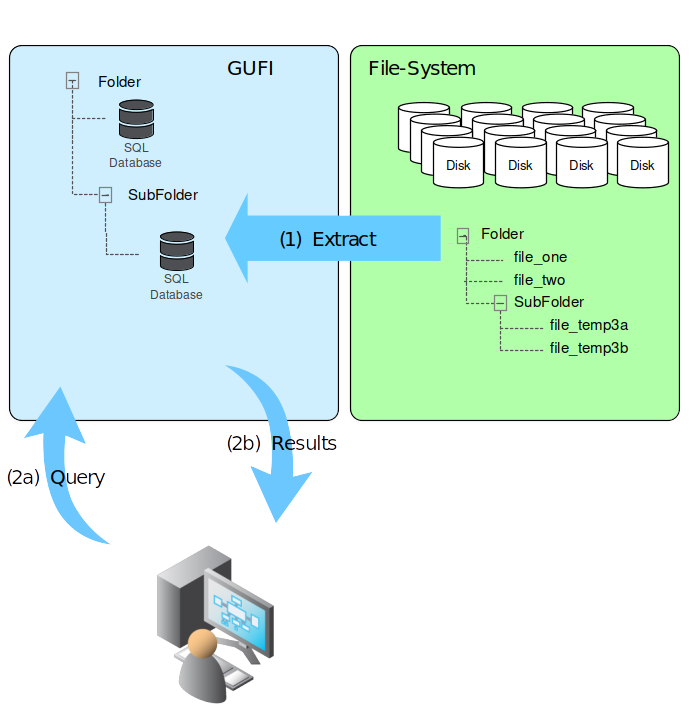
\includegraphics[width=0.5\textwidth]{gufi_structure.png}
\caption{\label{fig:gufi\_structure}Layout and user interaction with GUFI}
\end{figure}

\clearpage

\section{Understanding the data and how its stored}
The data stored in these databases include filenames, access and creation dates, file attributes, and extended attributes. Depending on which table is viewed and what view is selected, there can be up to 59 attributes(columns) per entry(row)\\
\\
Below are the most commonly used tables and views. 

\begin{figure} [h]
\centering
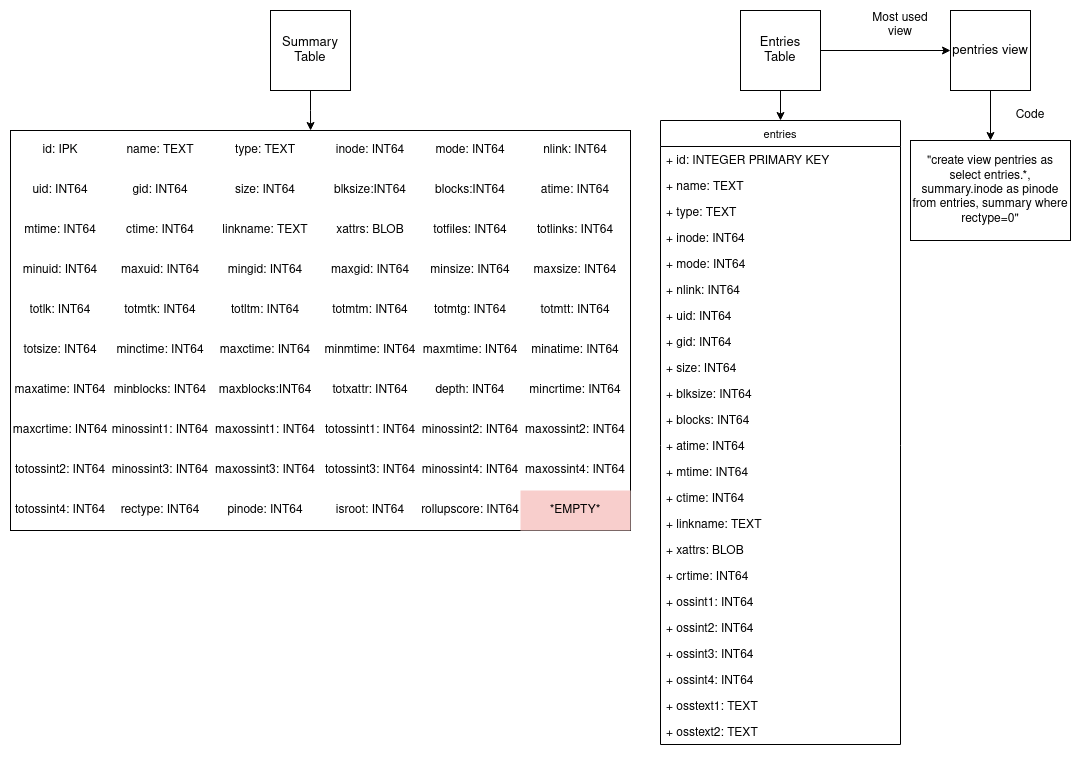
\includegraphics[width=1.0\textwidth]{Database_Schemas.png}
\caption{\label{fig:Database Schema}Database schema}
\end{figure}

\subsection{Why pentries is the most commonly used}
\begin{itemize}
  \item Provides parent inode as a query-able variable to the entries table
  \item Exists solely because parent inodes are not stored
  \item Parent inode is calculated/looked up so that parent inodes are never stored with child records.
\end{itemize}

\clearpage

\section{gufi\_query}

\subsection{Outline}

gufi\_query is used in order to query information from the generated databases that include all of the information about the indexed root directory and its sub-directories while also taking into account permissions 
\subsection{Flags}

\begin{table} [h]
\centering
\begin{tabular}{l|p{6cm}}
Flag & Functionality \\\hline
-h & help\\
\hline
-H & show assigned input values (debugging)\\
\hline
-E \textless SQL ent\textgreater & SQL for entries table \\
\hline
-S \textless SQL sum\textgreater (will be read first) & SQL for summary table\\
\hline
-T \textless SQL tsum\textgreater & SQL for tree-summary table\\
\hline
-a & AND/OR (SQL query combination)\\
\hline
-n \textless threads\textgreater & number of threads\\
\hline
-j & print the information in terse form\\
\hline
-o \textless out\_fname\textgreater & output file (one-per thread, with thread-id suffix) implies -e 1\\
\hline
-d \textless delim\textgreater & one char delimiter \\
\hline
-O \textless out\_DB\textgreater & output DB, implies -e 1 \\
\hline
-I \textless SQL\_init\textgreater & SQL init \\
\hline
-F \textless SQL\_fin\textgreater & SQL cleanup \\
\hline
-y \textless min-level\textgreater & minimum level to descend to \\
\hline
-z \textless max-level\textgreater & maximum level to descend to\\
\hline
-J \textless SQL\_interm\textgreater & SQL for intermediate results (no default: recommend using "SELECT * FROM entries") \\
\hline
-K \textless create aggregate\textgreater & SQL to create the final aggregation table (if not specified, -I will be used)\\
\hline
-G \textless SQL\_aggregate\textgreater & SQL for aggregated results (no default: recommend using "SELECT * FROM entries")\\
\hline
-e \textless 0 or 1\textgreater & 0 for aggregate, 1 for print without aggregating (implied by -o and -O)\\
\hline
-m & Keep mtime and atime same on the database files \\
\hline
-B \textless buffer size\textgreater & size of each thread's output buffer in bytes \\
\hline
-w & open the database files in read-write mode instead of read only mode
\end{tabular}
\caption{\label{tab:widgets}Flags and Arguments}
\end{table}

\clearpage

\subsection{Example Calls}

gufi\_query -S "SELECT * FROM summary" ~/directory\_of\_root\_index
\\
gufi\_query -E "SELECT * FROM pentries" ~/directory\_of\_root\_index


\subsection{Visualizing the Workflow}


\begin{figure} [h]
\centering
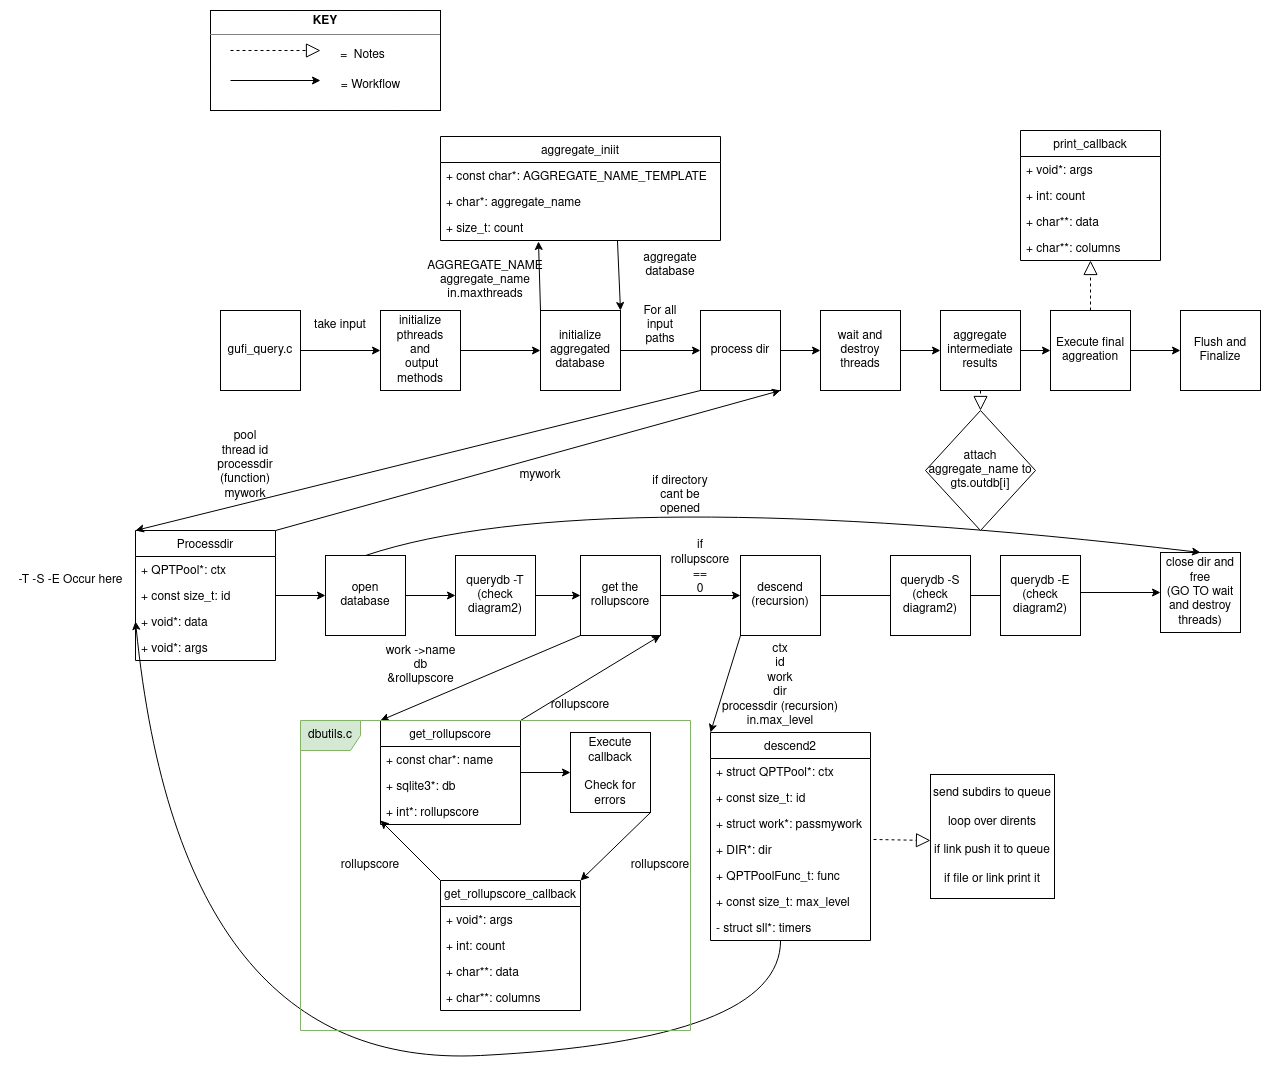
\includegraphics[width=1.0\textwidth]{gufi_query.png}
\caption{\label{fig:gufi_query}Workflow of gufi\_query}
\end{figure}

\subsection{Processdir}
What you will quickly notice when tracing through the above diagram (Figure 3) the major functionality from this code comes from the processdir function. This function is where the -E -S and -T flags are processed. Therefore, this is where all of the SQL database accesses occur. This process is parallelized via a thread pool and is further optimized by a calculated rollupscore to ensure that we only descend into necessary sub-directories.

\clearpage

\subsection{querydb}
querydb is the macro used to execute sqlite commands


\begin{figure} [h]
\centering
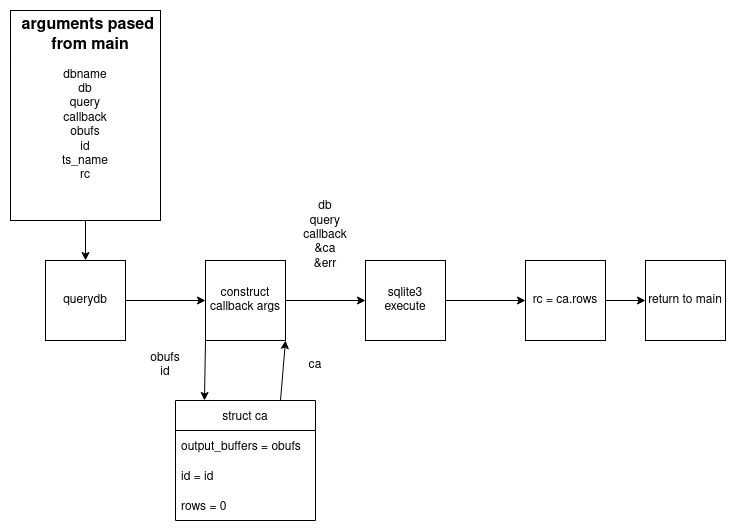
\includegraphics[width=0.8\textwidth]{querydb.png}
\caption{\label{fig:querydb}querydb workflow}
\end{figure}


\clearpage

\section{gufi\_dir2index}

\subsection{Outline}
gufi\_dir2index is used in order to turn a directory into a GUFI index. This process involves creating a database template that will be copied and modified for all directories and sub-directories as gufi descends down the tree. The information of the non-directories is stored inside of the databases. Permissions are established and any resulting errors establishing them are ignored

\subsection{Flags}

\begin{table} [h]
\centering
\begin{tabular}{l|r}
Flag & Functionality \\\hline
-h & help manual \\
-H & Show assigned input values \\
-n \textless num\_threads\textgreater  & define number of threads to use \\
-x & pull xattrs from source file-sys into GUFI \\
-z \textless max\_level\textgreater & maximum level to go down to
\end{tabular}
\caption{\label{tab:widgets}Flags and Arguments}
\end{table}

\begin{figure} [h]
\centering
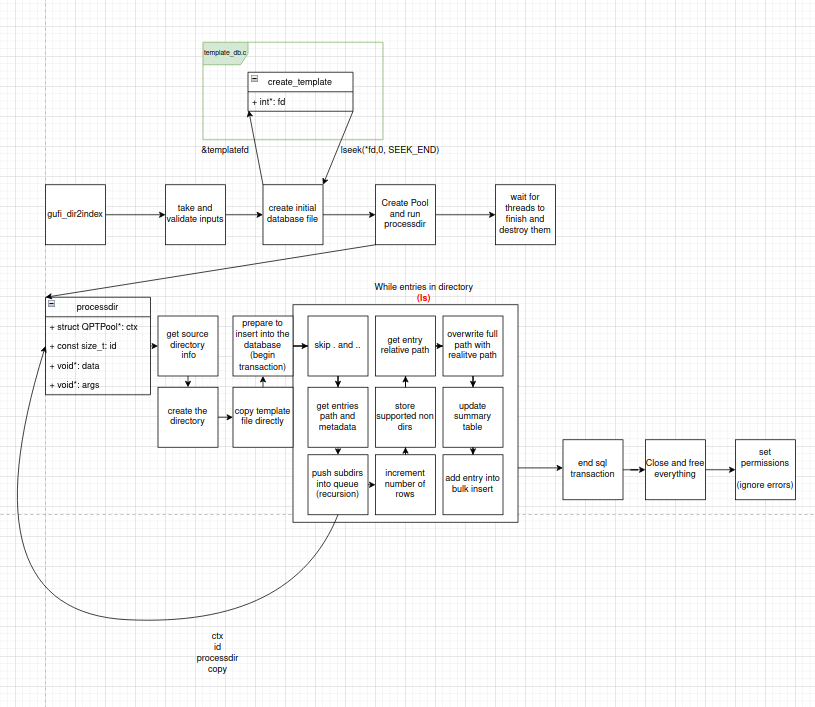
\includegraphics[width=1.0\textwidth]{gufi_dir2index.png}
\caption{\label{fig:gufi_dir2index}gufi\_dir2index workflow}
\end{figure}

\subsection{Usage}
gufi\_dir2index [flags] [directory to index] [location to place indexed directory]


\section{Understanding Rollup}
One of the predominant time savers in GUFI is the rollup feature which functions like so: \\
\begin{itemize}
  \item contents of the child's summary table are copied up with name column to include the parent directory
  \item pentries view/table is dropped and a pentries table is created with the data inside the pentries view/table
  \item copy child's pentries view into parent (regardless if view or table)
  \item ALL children must be able to rollup
\end{itemize}


\begin{figure} [h]
\centering
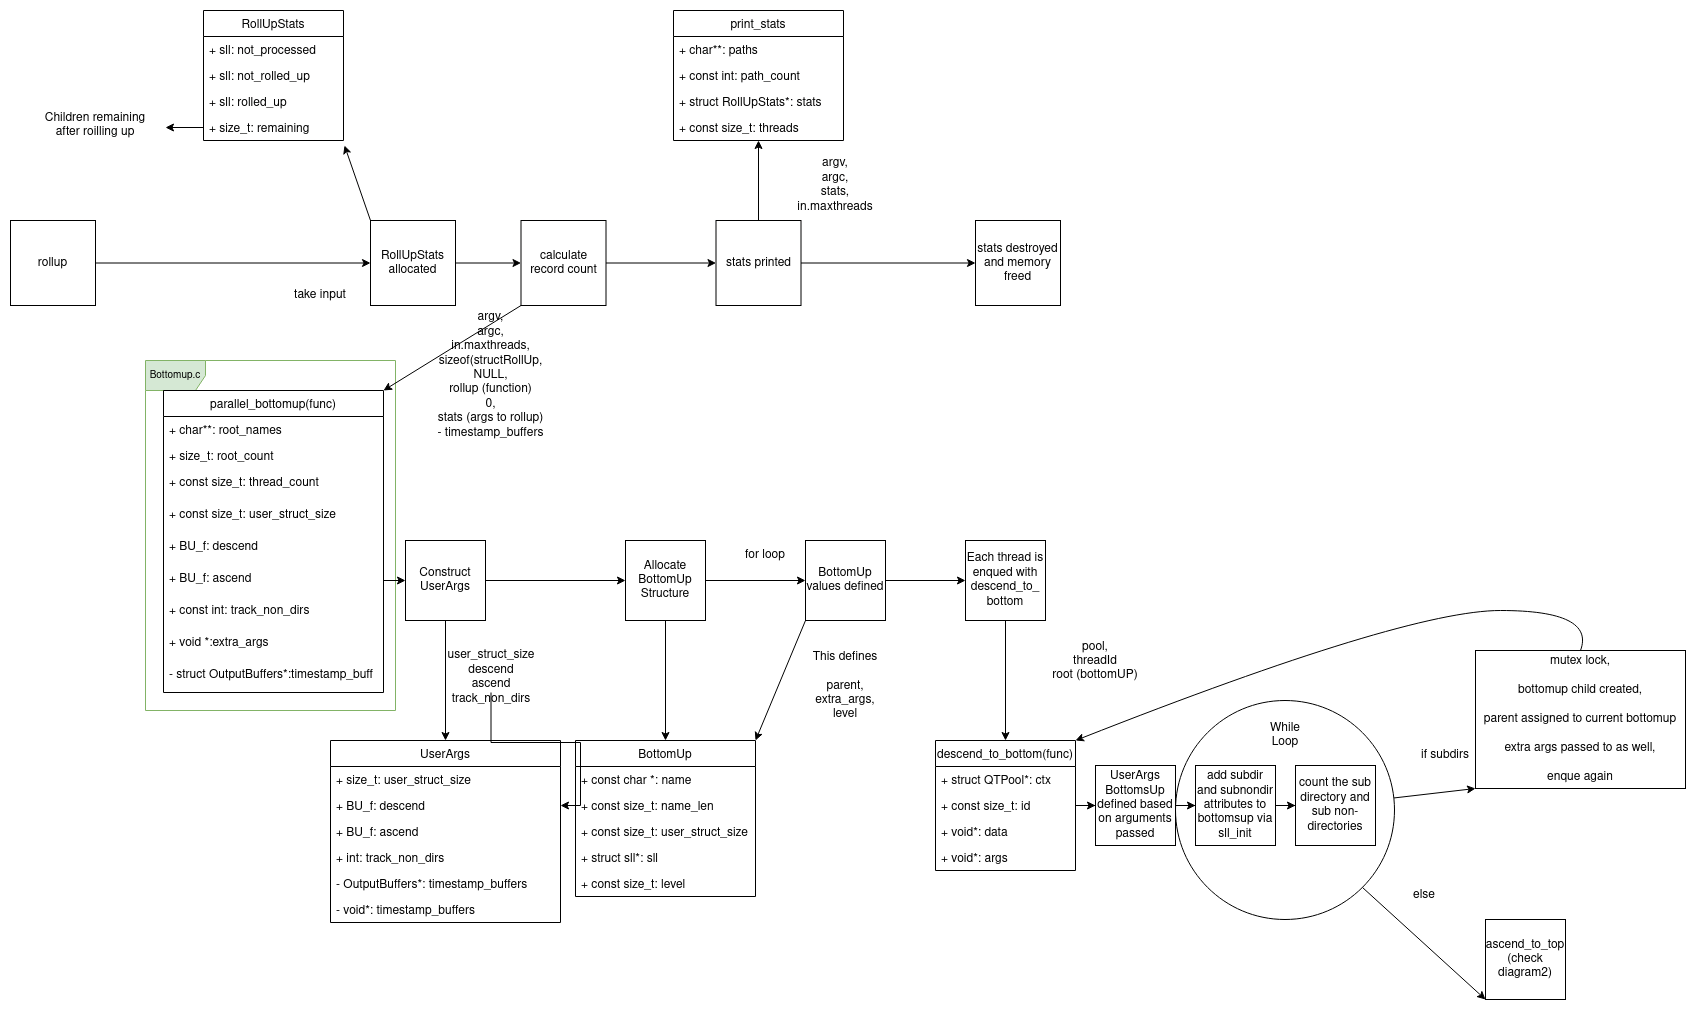
\includegraphics[width=1.2\textwidth]{rollup.png}
\caption{\label{fig:rollup}Rollup Workflow}
\end{figure}


\begin{figure} [h]
\centering
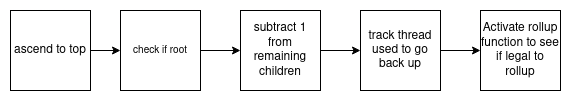
\includegraphics[width=0.8\textwidth]{ascending.png}
\caption{\label{fig:gufi_query} Ascending Workflow}
\end{figure}

\clearpage

\section{gufi\_dir2trace}
gufi\_dir2trace is to generate a trace of the files and directories inside of a specified root directory
\subsection{Flags}

\begin{table} [h]
\centering
\begin{tabular}{l|r}
Flag & Functionality \\\hline
-h & help manual \\
-H & Show assigned input values \\
-n \textless num\_threads\textgreater  & define number of threads to use \\
-x & pull xattrs from source file-sys into GUFI \\
-z \textless max\_level\textgreater & maximum level to go down to
\end{tabular}
\caption{\label{tab:widgets}Flags and Arguments}
\end{table}

\subsection{Usage}
gufi\_dir2trace [flags] [directory to trace] [prefix of output files]


\end{document}